\documentclass[border=5pt]{standalone}
\usepackage{tkz-euclide}
\usepackage{libertine}
\begin{document}

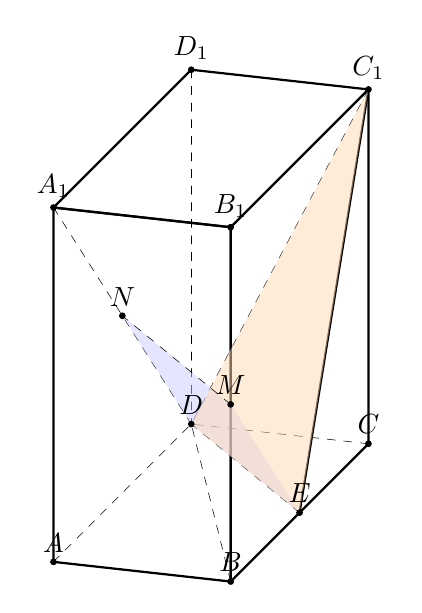
\begin{tikzpicture}
    \tkzDefPoints{0/0/A,2.25/-.25/B,4/1.5/C,1.75/1.75/D}
    \tkzDefPoints{0/4.5/A_1,2.25/4.25/B_1,4/6/C_1,1.75/6.25/D_1}
    \tkzDrawPolygons[thick](A_1,B_1,C_1,D_1 A,B,B_1,A_1 B,C,C_1,B_1)
    \tkzDefMidPoint(D,A_1) \tkzGetPoint{N}
    \tkzDefMidPoint(B,B_1) \tkzGetPoint{M}
    \tkzDefMidPoint(B,C) \tkzGetPoint{E}
    \tkzDrawSegments[thick](C_1,E)
    \foreach \i in {A,A_1,C,D_1,B,E,C_1}{
        \tkzDrawSegments[dashed](\i,D)
    }
    \tkzFillPolygon[blue!20,opacity=0.5](N,M,E,D)
\tkzFillPolygon[orange!30,opacity=0.5](C_1,E,D)
\tkzDrawSegments[dashed](M,N)
\tkzDrawPoints[black](A,B,C,D,A_1,B_1,C_1,D_1,E,M,N)
\tkzLabelPoints[above](A,B,C,D,A_1,B_1,C_1,D_1,E,M,N)
\end{tikzpicture}

\end{document}